插入并列的子图,共享标题
%\usepackage{subfigure}
%
%\begin{figure}[H]
%	\centering
%	\subfigure[SubfigureCaption]{
%		\label{Fig.sub.1}
%		\includegraphics[width=0.4\textwidth]{figurename.eps}}
%	\subfigure[SubfigureCaption]{
%		\label{Fig.sub.2}
%		\includegraphics[width=0.4\textwidth]{figurename.eps}}
%	\caption{MainfigureCaption}
%	\label{Fig.lable}
%\end{figure}


1. 并排摆放,共享标题
当我们需要两幅图片并排摆放,并共享标题时,可以在 figure 环境中
使用两个 \includegraphics 命令。
\begin{figure}[htbp]
	\centering
	\includegraphics[width=3in]{left}
	\includegraphics[width=3in]{right}
	\caption{中国富强}
\end{figure}
2. 并排摆放,各有标题
如果想要两幅并排的图片各有自己的标题,可以在 figure 环境中使用
两个 minipage 环境,每个环境里插入一个图。
\begin{figure}[htbp]
	\centering
	\begin{minipage}[c]{0.48\textwidth}
		\centering
		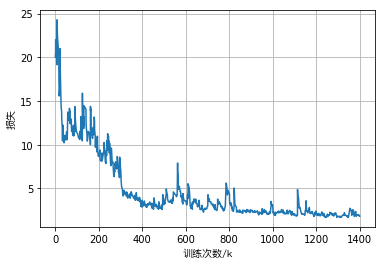
\includegraphics[width=3in]{figures/4_3_ft3d_loss}
		\caption{损失函数变化趋势}
	\end{minipage}
	\hfill
	\begin{minipage}[c]{0.48\textwidth}
		\centering
		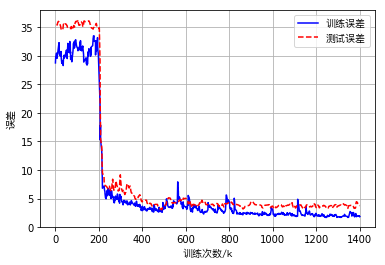
\includegraphics[width=3in]{figures/4_3_ft3d_error}
		\caption{训练/测试误差变化趋势}
	\end{minipage}
\end{figure}
3.并排摆放,共享标题,各有子标题
如果想要两幅并排的图片共享一个标题,并各有自己的子标题,可以使用 subfig 宏包提供的 \subfloat 命令。
subfloat 命令缺少宽度参数。虽然我们可以用 \hspace 命令调整子图的距离,子标题却只能和子图本身一样宽,就会出现折行。
为了避免子标题折行,我们可以在 \subfloat 里再嵌套个 minipage,因为后者是有宽度的。
\begin{figure}[htbp]
	\centering
	\subfloat[中国富强]{
		\label{fig:improved_subfig_a}
		\begin{minipage}[t]{0.3\textwidth}
			\centering
			\includegraphics{left}
		\end{minipage}
	}
	\subfloat[中国富强]{
		\label{fig:improved_subfig_b}
		\begin{minipage}[t]{0.3\textwidth}
			\centering
			\includegraphics{right}
		\end{minipage}
	}
	\caption{中国富强}
\end{figure}


通过minipage  生成的一个2*2图片排列的效果:
\begin{figure}
	%\begin{tabular}{cc}
	\begin{minipage}{0.48\linewidth}
		\centerline{\includegraphics[width=4.0cm]{a.eps}}
		\centerline{(a) Result 1}
	\end{minipage}
	\hfill
	\begin{minipage}{.48\linewidth}
		\centerline{\includegraphics[width=4.0cm]{a.eps}}
		\centerline{(b) Results 2}
	\end{minipage}
	\vfill
	\begin{minipage}{0.48\linewidth}
		\centerline{\includegraphics[width=4.0cm]{b.eps}}
		\centerline{(c) Result 3}
	\end{minipage}
	\hfill
	\begin{minipage}{0.48\linewidth}
		\centerline{\includegraphics[width=4.0cm]{b.eps}}
		\centerline{(d) Result 4}
	\end{minipage}
	%\end{tabular}
	\caption{Example of placing a figure with experimental results.}
	\label{fig:res}
\end{figure}